% !TeX spellcheck = fr_FR
\documentclass{article}
\usepackage[a4paper,pdftex]{geometry}
\usepackage[french]{babel}
\usepackage{xcolor}
\usepackage{fix-cm}
\usepackage{hyperref}
\usepackage[utf8]{inputenc} % Required for inputting international characters
\usepackage[T1]{fontenc} % Output font encoding for international characters
\usepackage{color,soul}
\usepackage{graphicx}
\usepackage{eurosym}
\usepackage{float}

\setlength{\oddsidemargin}{0mm} 
\setlength{\evensidemargin}{0mm} 
\newcommand{\HRule}[1]{\hfill \rule{0.2\linewidth}{#1}} % Horizontal rule at the bottom of the page, adjust width here

\definecolor{grey}{rgb}{0.9,0.9,0.9} % Color of the box surrounding the title - these values can be changed to give the box a different color	
\definecolor{umonsgreen}{rgb}{0.56862745,0.78039216,0.63137255}
\definecolor{umonsdarkgreen}{rgb}{0.4,0.47,0.42}
\definecolor{umonsblue}{rgb}{0.23,0.85,0.98}
\definecolor{umonsdarkblue}{rgb}{0.23,0.33,0.95}
\definecolor{umonsmetalblue}{rgb}{0.21,0.67,0.61}
\definecolor{umonsred}{RGB}{168, 0, 57}
\definecolor{umonsgray}{RGB}{150, 150, 150}
\definecolor{umonsturquoise}{RGB}{0, 171, 204}


\setul{0.3ex}{0.2ex}
%\setulcolor{umonsred}
\newcommand{\umonsU}{\textbf{\color{umonsgray}\setulcolor{umonsred}\ul{U}}}


\usepackage[backend=biber,style=numeric,natbib=true]{biblatex} % Use the bibtex backend with the authoryear citation style (which resembles APA)

\addbibresource{sources.bib} % The filename of the bibliography

\usepackage[autostyle=true]{csquotes} % Required to generate language-dependent quotes in the bibliography

\begin{document}

\thispagestyle{empty}

%----------------------------------------------------------------------------------------
%	TITLE SECTION
%----------------------------------------------------------------------------------------

\colorbox{umonsmetalblue}{
	\parbox[t]{1.0\linewidth}{
		\centering \fontsize{40pt}{80pt}\selectfont % The first argument for fontsize is the font size of the text and the second is the line spacing - you may need to play with these for your particular title
		\vspace*{0.7cm} % Space between the start of the title and the top of the grey box
		
		\hfill Questions théoriques \\
		\hfill Entrepreneuriat\\
		\hfill 2016-2017\par
		
		\vspace*{0.7cm} % Space between the end of the title and the bottom of the grey box
	}
}

%----------------------------------------------------------------------------------------

\vfill % Space between the title box and author information

%----------------------------------------------------------------------------------------
%	AUTHOR NAME AND INFORMATION SECTION
%----------------------------------------------------------------------------------------

{\centering \Large 
	\hfill Plein de gens \\
	\hfill Plein de sections \\
	\hfill {\fontfamily{ptm}\selectfont \umonsU \textcolor{umonsred}{MONS}} \\
	\hfill
	\href{mailto:t-as-vraiment-cliqué@pigeon.you}{Plein d'adresses mail} \\
	
	\HRule{1pt}} % Horizontal line, thickness changed here

%----------------------------------------------------------------------------------------

\clearpage % Whitespace to the end of the page
\setcounter{tocdepth}{1}
\tableofcontents
\clearpage % Whitespace to the end of the page

%todo: choppez une des sections (les "todos" suivants), certains ont 2 questions, d'autres 3 mais a priori certaines questions sont plus faciles donc ça devrait être +/- réparti équitablement. Petit conseil: mettre des dessins accompagnés d'explications(un dessin est plus facile à retenir qu'un texte). Bon site pour faire des schémas: https://www.draw.io/

%todo EMILIEN PERETTI
\section{Quels sont les points (contenu) à aborder lors du pitch et que doit contenir un executive summary ?}
Le but du pitch est de donner envie à l'interlocuteur de découvrir notre "Executive
Summary". Celui-ci doit comporter la réponse aux questions suivantes: 
\begin{itemize}
\item Qui vous êtes et comment vous contacter ?
\item Quel est le problème que le produit / service résout ?
\item Quel est la valeur ou le bénéfice qu’il apporte ?
\item Pourquoi est-ce important et excitant?
\item Qu’avez-vous déjà accompli et de quoi avez-vous besoin pour réussir ?   
\end{itemize}
L'Executive Summary,quant à lui, a pour but d'obtenir une invitation pour présenter le projet et donner envie de lire le plan financier. Il doit contenir les points suivants:
\begin{itemize}
\item Origine du projet
\item Résumé de la solution proposée
\item Marché
\item Stratégie
\item La société et l’équipe
\item Concurrence et avantage compétitif
\item Synthèse stratégie et plan d’actions
\item Principaux chiffres (chiffre d'affaire, bénéfice, cashflow, investissements et besoins financiers)
\end{itemize}
\section{Quelle est la structure classique d’un plan d’affaires ?}
Le structure classique d'un plan d'affaires est la suivante:
\begin{enumerate}
\item Définition du projet et de l’historique
\item L’équipe
\item La solution «produit/service»
\item Le(s) marché(s)
\item La concurrence
\item La vision – La stratégie et les objectifs – Le  plan d’action
\item Les besoins financiers (plan financier)
\item La proposition d’investissement
\end{enumerate}

\section{Quels sont les 2 différents aspects à traiter pour le marché, et à quelles questions doit-on répondre?}

%%%%%%%%%%%%%%%%%%%%%%%%%%%%%%%%%%%%%%%%%%%%%%%%%%%%%%%%%%%%%%%%%%%%%%%
%todo: Duncan
\section{Définissez Marché, segment de marché et niche.}
\begin{tabular}{|rcl|}
\hline
&&\\
Marché & : & TODO\\ %TODO
&&\\
\hline
&&\\
&& \multicolumn{1}{p{.8\textwidth}|}{Définition simple: "Regroupement homogène de personnes (selectionnées sur de nombreux critères) sur lesquelles il est possible d'effectuer des actions marketing de différenciations."}\\
Segment de Marché & : & \multicolumn{1}{p{.8\textwidth}|}{En gros, on peut segmenter le marché global en plus petits groupes sur lesquels la publicité (marketing) va pouvoir effectuer des actions ciblées. Par exemple, un grand nombre de gens aiment le coca cola mais en segmentant le marché des consommateurs par âge, coca peut par exemple faire ses campagnes pub "fun et fête" en visant le segment 15-30 ans. Ou la pub de Noël qui est plutôt pour les enfants (magique, papa noël, toussah,...)}\\
&&\\
\hline
&&\\
Niche & : & \multicolumn{1}{p{.8\textwidth}|}{Petite maison pour chien généralement placée dans le fond du jardin.}\\
&&\\
\hline
&&\\
				 &   & \multicolumn{1}{p{.8\textwidth}|}{Un marché de niche est un marché très étroit correspondant à un produit ou service très spécialisé.}\\
Marché de Niche & : & \multicolumn{1}{p{.8\textwidth}|}{Le fait de viser un marché de niche permet souvent d’être confronté à une concurrence moins forte et à un potentiel de marges plus élevées, mais les volumes de ventes potentiels sont naturellement plus faibles et limités.}\\
				 &  & \multicolumn{1}{p{.8\textwidth}|}{Le caractère de niche de marché est une notion très relative selon les contextes. Un marché de niche peut être de quelques centaines de milliers d’euros ou de quelques millions, voire dizaines de millions d’euros, si on se trouve dans le domaine du marché automobile.}\\
				 &  & \multicolumn{1}{p{.8\textwidth}|}{En gros, Un marché de niche c'est donc un marché qui va intéresser des gens cherchant un produit très particulier. Une entreprise se lançant actuellement dans la vente de fusées pour aller sur la lune VA se trouver sur un marché de Niche (enfin je pense pas que beaucoup de gens veulent acheter des fusées lunaires) Alors vu que c'est un marché avec peu de clients ben d'un côté on va pas avoir beaucoup de ventes mais de l'autre on peut fixer le prix et/car la concurrence est faible.}\\
&&\\
\hline
\end{tabular}
\section{Que faut-il comprendre / analyser dans l’offre des concurrents et pourquoi ?} %TODO
Il faut comprendre et analyser leur avantages et désavantages par rapport à notre entreprise, ceci peut se faire via \textbf{le canevas stratégique} \ref{fig:canevasStrategique}
\begin{figure}[H]
	\centering
	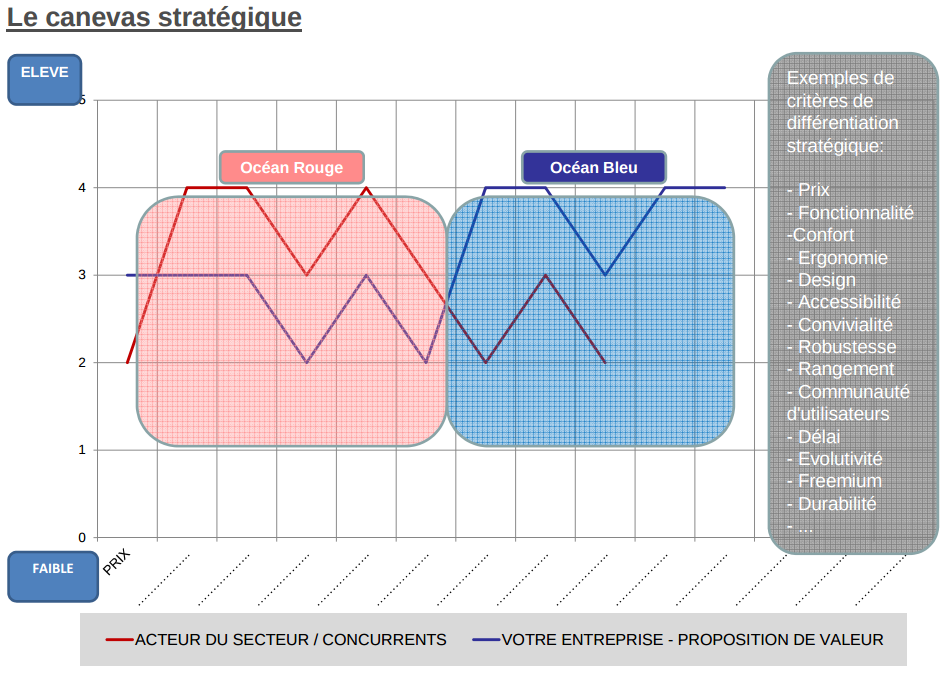
\includegraphics[width=14cm]{canevasStrategique.png}
	\label{fig:canevasStrategique}
\end{figure}
\section{Quels sont les objectifs du plan financier ?} %TODO


%%%%%%%%%%%%%%%%%%%%%%%%%%%%%%%%%%%%%%%%%%%%%%%%%%%%%%%%%%%%%%%%%%%%%%%
%todo: Adrien
\section{Quelles sont les différentes mesures de la rentabilité des investissements ? Détaillez-en une.}
\subsection{VAN}
\begin{figure}[H]
	\centering
	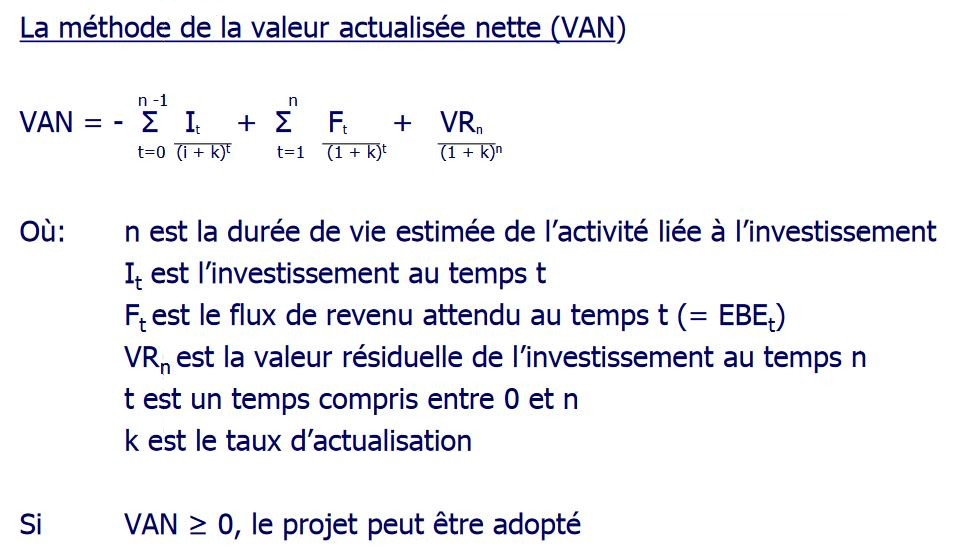
\includegraphics[width=14cm]{van.jpg}
\end{figure}

\paragraph{Un exemple pratique:}
Une entreprise envisage l’acquisition d’une machine d’une valeur de 10.000\euro{}, utilisable et amortissable en linéaire sur 5 ans.
Au bout des 5 ans, elle pourra encore être revendue à 1.000\euro{}.
Cette machine permettrait d’améliorer le chiffre d’affaires de 7.000\euro{} par an et augmenterait les coûts de 2.000\euro{} par an. Le taux d’ actualisation retenu est de
10\%. 30\% d’impôts. Cet investissement peut-il être envisagé ? (voir table \ref{van})

\begin{table}[H]
	%\begin{center}
\begin{tabular}{l c r}
	chiffre d’ affaires supplémentaire &=&	7.000 \euro{}\\
	- coût supplémentaire	&=&	-2.000 \euro{} \\
	\hline
	résultat brut généré	&=&	5.000 	\euro{}\\
	- amortissements	&=&	-2.000 	\euro{}\\
	\hline
	résultat d’	exploitation	&=&	3.000 \euro{}\\
	- impôts (30\%)	&=&	-900 	\euro{}\\
	\hline
	\color{red}résultat net	&\color{red}=&	\color{red}2.100 	\euro{}\\
	+ amortissements	&=&	+2.000 	\euro{}\\
	\hline
	\color{red}F	&\color{red}=&	\color{red}4.100 	\euro{}\\
\end{tabular}
%\end{center}
\caption{\label{van} Calcul du Flux de Revenus (F) hors économie fiscale}
\end{table}

Donc, l’investissement rapporte :
\begin{itemize}
	\item en année 1 : $F_1$ = -5.900 \euro{}
	\item en année 2 : $F_2$	= 	4.100 \euro{}
	\item en année 3 : $F_3$	= 	4.100 \euro{}
	\item en année 4 :	$F_4$	= 	4.100 \euro{}
	\item en année 5 : $F_5$	= 	4.100 	\euro{}
	\item en année 5 : la valeur résiduelle de la machine, soit, $1000 (1-0,30) = 700$ \euro{}
\end{itemize}
\begin{figure}[H]
	%\centering
	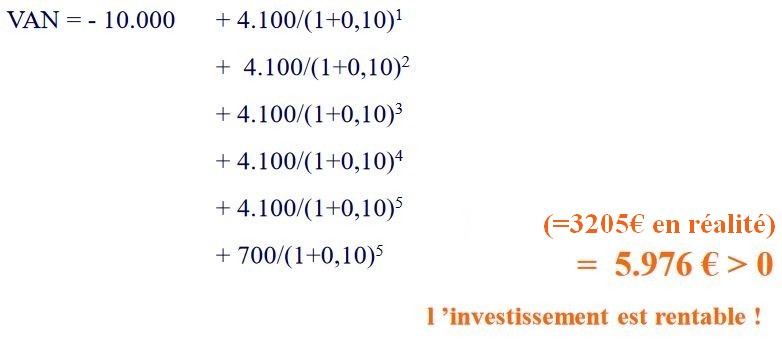
\includegraphics[width=10cm]{van-rentabilite.jpg}
\end{figure}

\subsection{TRI}

\begin{figure}[H]
	\centering
	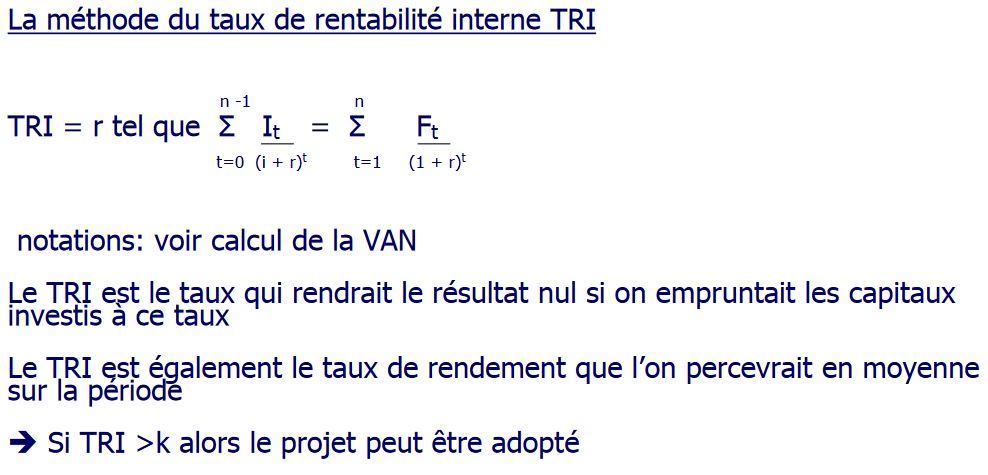
\includegraphics[width=14cm]{tri.jpg}
\end{figure}

Sur l'exemple:

\begin{figure}[H]
	%\centering
	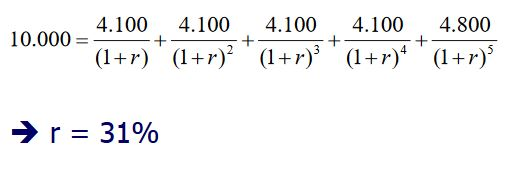
\includegraphics[width=10cm]{tri-exemple.jpg}
\end{figure}

Notes : 
Une tentative de graphe est dispo dans les slides sur la relation entre TRI et VAN mais ne veut absolument rien dire (si ce n'est mettre en évidence le fait que VAN=\euro{} et TRI=\%).
Les slides présentent aussi la méthode PRA pour évaluer le temps nécessaire pour récupérer les montants investis mais précise que ça ne mesure pas la rentabilité du projet (malgré que ça se trouve dans la section rentabilité des investissements).

\section{Quelle est la principale mesure de la rentabilité de l’exploitation ? Quelles en sont les limites ?}

\subsection{BEP}
Le seul de rentabilité (break-even point, BEP). Il répond à la question \textquote{quelle doit être la quantité à produire et à vendre de telle manière que les revenus (c’est-à-dire le chiffre d’affaires) couvrent l’ensemble des coûts?}. Au moment où on l'atteint, il n'y a ni gain, ni perte.

\begin{figure}[H]
	%\centering
	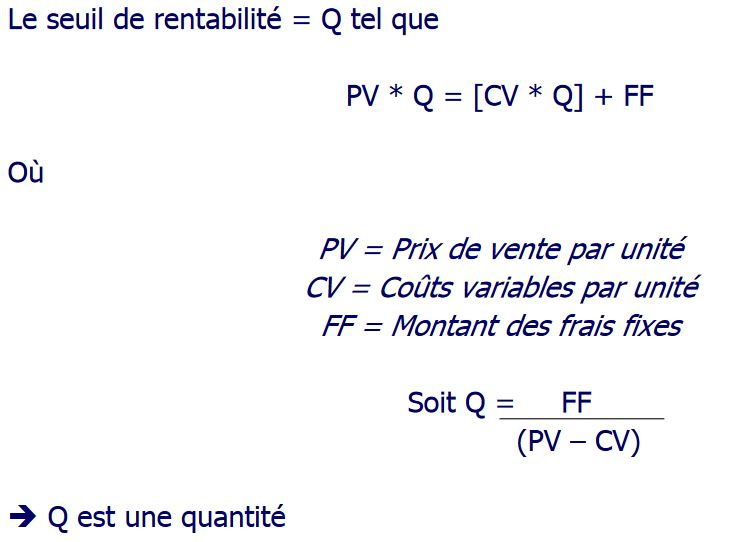
\includegraphics[width=10cm]{bep.jpg}
\end{figure}

\begin{figure}[H]
	\centering
	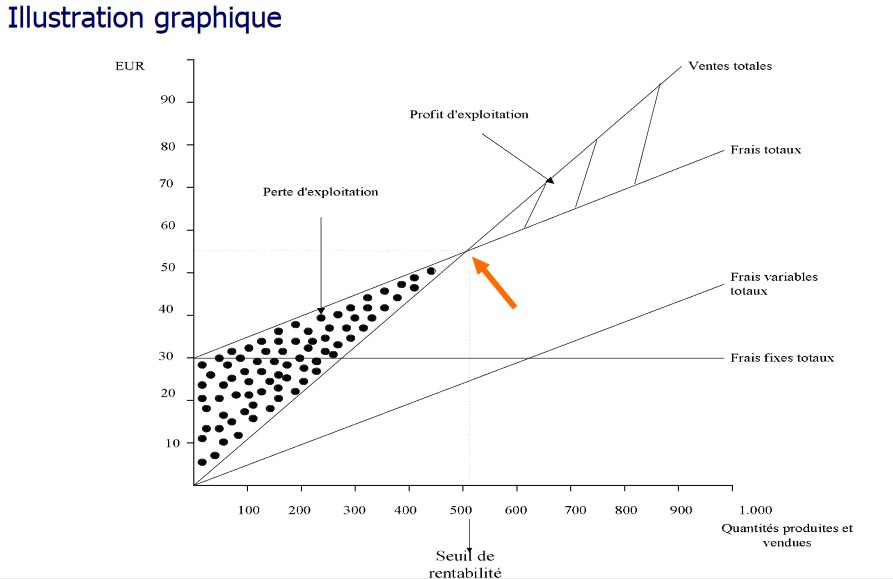
\includegraphics[width=10cm]{bep-graphe.jpg}
\end{figure}

\subsection{Ses limites}
Les limites de l’approche «seuil de rentabilité» :
\begin{itemize}
	\item Les prix de vente et les coûts variables unitaires sont-ils constants dans 
	le temps et indépendants du volume?
	\item Comment appliquer la méthode quand on fait face à des produits 
	multiples, complémentaires ou substituables?
	\item Les frais fixes sont-ils constants dans le temps et réellement
	indépendants du volume de production/vente?
\end{itemize}
~\\
$\rightarrow$ Notion essentiellement de court terme. Elle suppose:

\begin{itemize}
	\item des investissements donnés,
	\item Un product mix donné,
	\item De faibles variations en termes de volume.
\end{itemize}

%%%%%%%%%%%%%%%%%%%%%%%%%%%%%%%%%%%%%%%%%%%%%%%%%%%%%%%%%%%%%%%%%%%%%%%
%todo: 4
\section{Définissez le BFR et pourquoi faut-il surveiller son évolution ?}
\section{Citez des actions permettant d’améliorer la position de trésorerie d’une entreprise ?}


%%%%%%%%%%%%%%%%%%%%%%%%%%%%%%%%%%%%%%%%%%%%%%%%%%%%%%%%%%%%%%%%%%%%%%%
%todo: 5
\section{Expliquez les trois concepts essentiels analysés lors d’un diagnostic financier.}
\section{Définissez la notion de Valeur Ajoutée.}
\section{Qu’est ce que le cash flow d’une entreprise ou pourquoi est-ce vital ?}

\printbibliography

\end{document}